\documentclass[12pt]{article}

%Paquetes a utilizarse
\usepackage[width=7in, height=9.5in, top=0.75in, papersize={8.5in,11in}]{geometry}
\usepackage[spanish]{babel} 
\decimalpoint
\usepackage[utf8]{inputenc}
\usepackage{bbding}
\usepackage[colorlinks = true, linkcolor = blue, urlcolor = BlueViolet, citecolor = OliveGreen]{hyperref}
\usepackage{graphicx}
\usepackage{amssymb,amsthm,amsmath}
\usepackage{enumerate}
\usepackage{array,multicol,multirow}
\usepackage{xcolor}
\usepackage{fancybox,tcolorbox}
\usepackage{caption,subcaption,float,tabularx}
\usepackage{enumitem}

\theoremstyle{definition}
\newtheorem{corolario}{Corolario}
\newtheorem{lema}[corolario]{Lema}
\newtheorem{proposicion}[corolario]{Proposición}
\newtheorem{teorema}[corolario]{Teorema}
\newtheorem{propiedad}[corolario]{Propiedad}
\newtheorem*{observacion}{Observación}
\newtheorem{definicion}{Definición}
\newtheorem*{demostracion}{Demostración}
\newtheorem{ejemplo}{Ejemplo}
\newtheorem{problema}{Problema}
\newtheorem*{solucion}{Solución}
\newtheorem{ejercicio}{\PencilRightDown \  Ejercicio}
\newtheorem{step}{Paso}
\newtheorem{credito}{Crédito}

\usepackage{tikz}
\usetikzlibrary{arrows.meta,babel,calc,positioning}

\renewcommand{\arraystretch}{1.5}
\providecommand{\abs}[1]{\lvert#1\rvert}
\providecommand{\norm}[1]{\lVert#1\rVert}

\renewcommand{\tabularxcolumn}[1]{m{#1}}
\newcommand{\Evaluacion}[4]{
\setcounter{ejercicio}{0}
\noindent\begin{tabular}{lcr}
	\includegraphics[height=3cm]{Logos/logo-UES.png}\hspace{2.5em}
	&
	\includegraphics[height=2.75cm]{Logos/logo-PJT.png}
	& 
	\hspace{2.5em}\includegraphics[height=2.75cm]{Logos/logo-MINEDUCYT.png}
\end{tabular}

\hfill

\begin{center}
    
    UNIVERSIDAD DE EL SALVADOR
    \\PROGRAMA JÓVENES TALENTO
    \\FDTC 2022
    \\#2
    \\Nivel Olímpico C de Matemáticas

\end{center}

\begin{center}
    #1
\end{center}

%\textbf{Nombre}: \enspace\hrulefill

#3

\input{#4}
\newpage
}

\newtheorem{obs}{Observación}

%\usepackage[margin=2.5cm]{geometry}
%\usepackage{wasysym}
%\usepackage{stmaryrd,textcomp}
%\usepackage{pgf,tikz}
%\usetikzlibrary{arrows}

\parskip = 2mm   %%%% genera un espacio de X mm entre lo párrafos
\parindent = 3mm
\usepackage{multicol}
\usepackage{iwona}

\newcommand{\tema}{Intruducción}
\newcommand{\fecha}{Martes, 3 de Diciembre de 2024}
\newcommand{\sesion}{Corto 1}

\begin{document}
%\thispagestyle{empty}
%\newpage
\thispagestyle{empty}

\begin{figure}[h] 
	\begin{minipage}[b]{0.26\textwidth}
		\begin{center}
			
\includegraphics[height=3cm]{../Logos/UES.png}
			\par\end{center}
	\end{minipage} 
	\begin{minipage}[b]{0.46\textwidth}
		\begin{center}
			UNIVERSIDAD DE EL SALVADOR\\ [0.1cm]
			PROGRAMA JÓVENES TALENTO\\ [0.1cm]
	        FDTC 2024\\ [0.1cm]
                NIVEL 5\\ [0.1cm]
			COMBINATORIA 
			\par\end{center}
	\end{minipage} 
	\begin{minipage}[b]{0.05\textwidth}
		\begin{center}
			
\includegraphics[height=2cm]{../Logos/LOGO PJT.png}
			\par\end{center}
	\end{minipage}
\end{figure}

\begin{center}
    \begin{tabular}{p{4.5cm} p{7cm} p{4.5cm}}
        \tema & \centering\fecha & \hfill\sesion
    \end{tabular}
\end{center}
Nombre: \rule{15cm}{1pt}\newline

\textbf{INDICACIONES:} Resuelve cada problema de manera clara y ordenada, dejando constancia de tus procedimientos.
\begin{enumerate}
    \item (25\%) Dado el siguiente diagrama de Venn, encuentre $(A^c\cap B)-(B\cap C)$
    \begin{figure}[h]
        \centering
        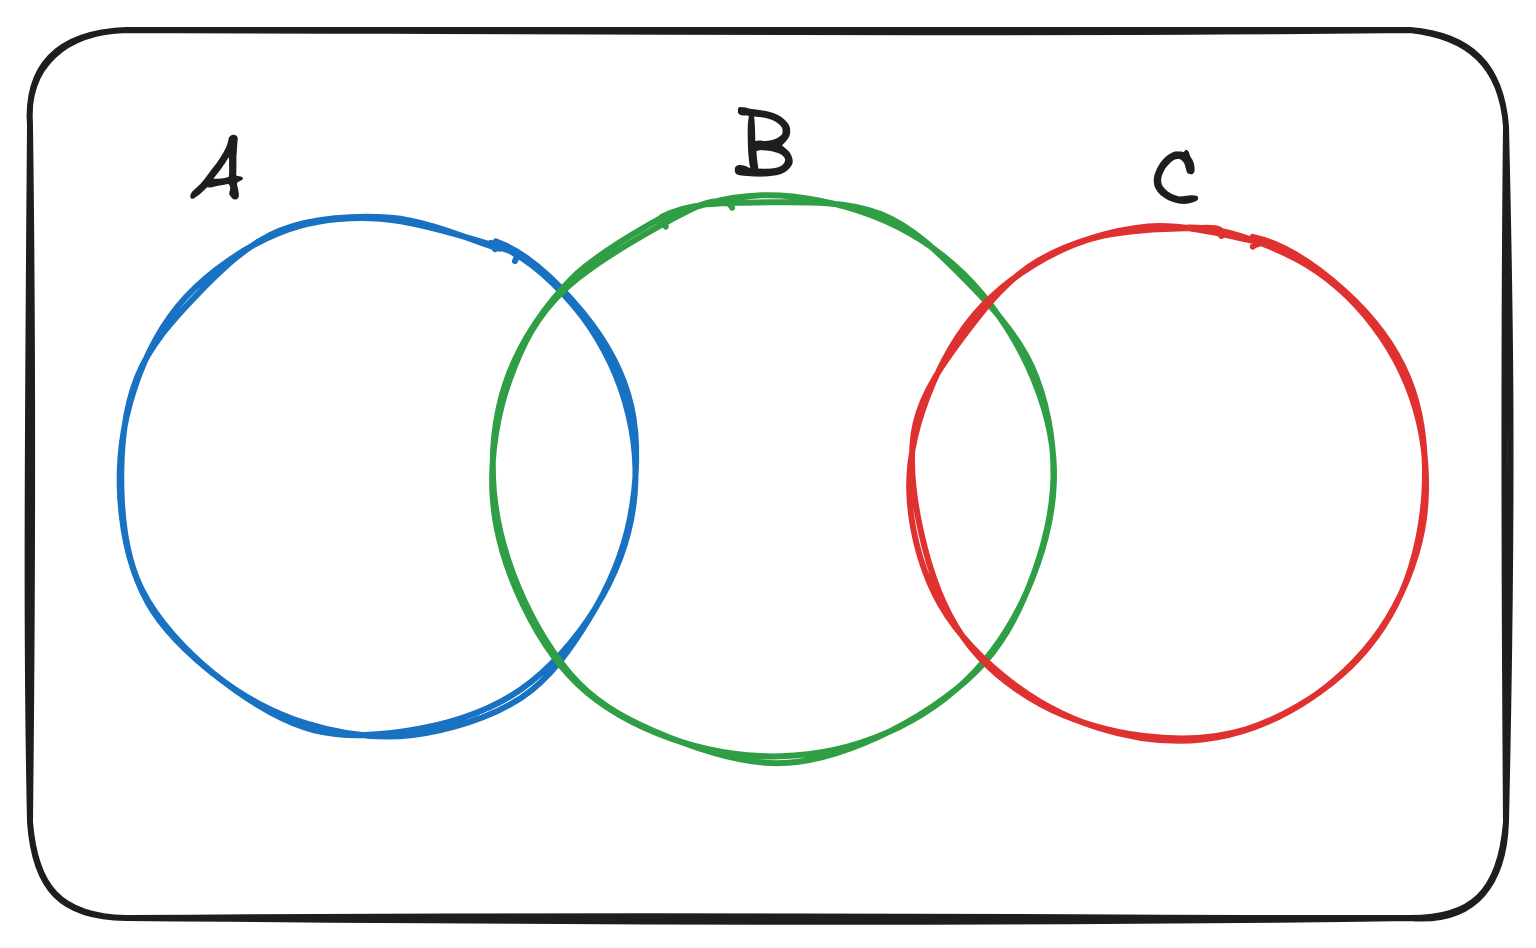
\includegraphics[width=0.3\textwidth]{../Imagenes/IMG1/venn.png}
        \caption{}
        \label{fig:enter-label}
    \end{figure}
    \item (25\%) Realize las siguientes operaciones con los conjuntos $A$, $B$ y $C$. Justifique cada operación.\[A=\{2n + 1 | n \in \mathbb{Z}\}\]\[B=\{x | -2 \leq x < 5\}\]\[C=\{-\pi, -e, \sqrt{2}, 1, 0, -1, \sqrt{3}, \sqrt{49}\}\]
    \begin{multicols}{2}
        \begin{enumerate}
        \item $(A\cap B)\cup C$.
        \item $(\mathbb{Q}\cap C)\cap B$.
        %\item $((A\cup B)\cap C)\cap \mathbb{R}$.
        %\item $((A-B)\cup (C-A))\cap (B-C)$.
        \item $((C-B)\cap A)-\mathbb{Z}$.
    \end{enumerate}
    \end{multicols}
    %\item (25\%) ¿Cuántos números de tres dígitos $abc$ son tales que $a+3b+c$ es múltiplo de 3?
    \item (25\%) Una cerradura de combinación está numerada del 0 al 30. Una combinación consta de tres números tal que dos números consecutivos deben ser diferentes, pero el primero y el tercero pueden ser iguales. ¿Cuántas combinaciones diferentes son posibles?\\
    \textbf{Ejemplo:} Una combinación válida es 30 29 30.
    \item (25\%) ¿Cuantos divisores positivos tiene 2024000000?
\end{enumerate}

\textbf{Crédito Extra:} En Braille se utiliza como base un rectángulo de $3\times2$, en el que en cada casilla se puede colocar un punto en relieve o dejar vacía. Si cada combinación de puntos y vacíos representa un carácter, ¿cuántos caracteres se pueden representar? (un carácter es un símbolo, como una letra o un número)


%Hay cuatro botes en una de las orillas de un río; sus nombres son Ocho, Cuatro, Dos y Uno, porque esa es la cantidad de horas que se tarda cada uno de ellos en cruzar el río. Se puede amarrar un bote a otro pero no más de uno, y entonces el tiempo que tardan en cruzar es igual al más lento de los dos botes. Un sólo marinero debe de llevar todos los botes a la otra orilla. Es decir, que un bote no puede cruzar sin marinero y el marinero viaja con uno o dos botes. ¿Cuál es la menor cantidad de tiempo que necesita el marinero para completar el traslado?

\end{document}